\documentclass[14pt]{report}
\title{The Future of Work: \\ Machine Learning and Employment}
\author{Mu Chen}

\usepackage[margin=0.787in]{geometry}

%\usepackage{fontspec}
%\setmainfont{Arial}
\usepackage{setspace}


\usepackage{cite}
\usepackage{adjustbox}
\usepackage[font={small}, labelfont = {bf}]{caption}
\usepackage{graphicx}
\usepackage{array}
\usepackage{subcaption}
\usepackage{amsmath}
\usepackage{amssymb}
\usepackage{setspace}
\usepackage{gensymb}
\usepackage{tablefootnote}
\usepackage[T1]{fontenc}
\usepackage{helvet}
\usepackage[utf8]{inputenc}
\usepackage{subcaption}
\usepackage{float} 
\usepackage{subfloat} 

\renewcommand{\familydefault}{\sfdefault}

\renewcommand{\thefootnote}{\roman{footnote}}
\renewcommand{\bibname}{References}

\newcounter{FootnoteCounter} 
\stepcounter{FootnoteCounter} % Add one to counter (initialised at zero)
%\footnotemark[\arabic{FootnoteCounter}] // Place the footnote number in the text
%\footnotetext[\arabic{FootnoteCounter}]{Example footnote} // Set the text to be displayed with this instance of footnote
%\stepcounter{FootnoteCounter} // Increment the counter for the next useage.

\usepackage{fancyhdr}
 
\usepackage{pdfpages}
 
 
\pagestyle{fancy}

\fancyfoot[C]{\sffamily\fontsize{9pt}{9pt}\selectfont\thepage}

\setlength{\textfloatsep}{\baselineskip + 0.2\baselineskip - 0.1\baselineskip}

\numberwithin{equation}{chapter}
\doublespace


\begin{document}
\pagenumbering{roman}
\newpage
\maketitle
\section*{Abstract}

\newpage
\section*{Acknowledgement}

\newpage 
\rhead{Table of Contents}
\lhead{} 
 
\tableofcontents

\begin{spacing}{2}

\newpage
\pagenumbering{arabic}
\setcounter{page}{1}



\chapter{Introduction}
\rhead{Introduction}
The question of how technology could influence employment has been a popular issue for quite a long time\cite{machin1998}. Since 1990s, it was believed that technological changes have favoured the more skilled workers while reduced the demand for less skilled workers\cite{bound1989changes}. Nowadays, with much faster development of technologies especially in automation technology, it is very reasonable to say that less human worker is required. If it is true, could it be the major cause for lower employment rate? Will the development of technology make more people jobless? Or is it just a temporary phenomenon? This report presents how these questions are answered using machine learning techniques...

(More to go depending on future experiments)



\newpage
\chapter{Gaussian Process}
\rhead{Gaussian Process}
Gaussian Process(GP) is a class of distributions in which each input space follows a Gaussian distribution and any finite combination of input spaces also has a joint Gaussian distribution. Each input represents an input space and therefore the distribution of Gaussian Process can be seen as the infinite-dimensional generalization of multivariate normal distributions. 

Gaussian Process has several advantages over other models. First, they are non-parametric, meaning no prior model is required for learning. Second, Gaussian Process is particularly useful for small data sets because the prescence of hyper-parameters gives it characteristics you want (such as smoothness and periodicity), at the same time keeping a fine fit to the data.  

By definition, a Gaussian Process $f(x)$ is specified by a mean function and a covariance function, denoted as  

\[f(x) \sim GP(\mu(x),K(x,x))\]

where

\begin{align}
\mu(x) &= \mathbb{E}(f(x))\\
k(x,x\prime) &= \mathbb{E}((f(x) - \mu(x)(f(x\prime) - \mu(x\prime)) 
\end{align}

Both the mean and covariance function are the choice of user and can have crucial effects on the final Gaussian process distribution.

To describe how all the input points are related together we use the covariance matrix defined as 

\begin{equation}
K(x,x\prime) = \left[\begin{array}{cccc}
k(x_1,x_1) & k(x_1,x_2) & \cdots & k(x_1,x_n)\\
k(x_2,x_1) & k(x_2,x_2) & \cdots & k(x_2,x_n)\\
\vdots & \vdots & \ddots & \vdots\\
K(x_n,x_1) & k(x_n,x_2) & \cdots & k(x_n,x_n)\\

\end{array}\right]
\end{equation}

\subsubsection{Mean Function}
The prior mean function $\mu(x)$ describes the beliefs in output y(x) before any observations are made. The most popular choices of $\mu$ includes 0 and other constants. More complicated mean functions can be defined by using certain parameters based on domain knowledge. However, one should always be careful in selecting the mean function since it is what our inference is extrapolated from.   

\subsubsection{Covariance Function}
Many characteristics such as smoothness, stationarity, and periodicity can be integrated in covariance function. It describes how individual observations are related to each other. In reverse, learning in Gaussian Process also defines the properties of covariance function, giving us the model that can be used for upcoming predictions.   

One common choice is the squared exponential covariance function
\[k(x,x\prime) = \sigma_f^2\operatorname{exp}\left[-\frac{(x-x\prime)^2}{2l^2}\right]\]
where $l$ is the lengthscale representing how far a certain training point could affect the predictions. It is suitable for smooth data. One thing to notice is that the $k(x,x\prime)$ is actually the covariance between $y$ and $y\prime$, corresponding to the output of $x$ and $x\prime$ respectively. Other covariance functions such as rational quadratic function can be useful for data that is smooth over a range of length scales.

Matérn class of covariance functions is another important branch of covariance functions. They take the form of 
\[K_{Matérn}(x,x\prime) = \lambda^2 \frac{2^{1-\nu}}{\Gamma(\nu)}\left(\frac{\sqrt{2\nu} d(x,x\prime)}{l}\right)^\nu K_\nu \left(\frac{\sqrt{2\nu} d(x,x\prime)}{l}\right)\]
where $d(x,x\prime)$ is the distance between $x$ and $x\prime$

They are used for functions of varying smoothness. 

Periodicity can be added by using the periodic covariance of the form
\[K_P(x,x\prime) = \lambda^2 \operatorname{exp}\left(- \frac{2sin^2\left(\pi d(x,x\prime)/\rho\right)}{\omega}\right)\] 
where $\rho$ determines the period and $\omega$ gives the roughness.

Covariance functions can be combined to give multi-character correlations. For example, if we know that it requires both periodicity and smoothness in the distribution, the multiplication of squared exponential function and periodic function can be used. If the prior information is that either periodicity or smoothness exists, the addition of the above two functions suits better. Similar techniques can be applied to distributions that are known to be the sum of independent functions or the product of independent functions.

One thing to notice is that most of the covariance functions involves computing the distance between input points. This distance could either simply be the euclidean distance $d_E(x,x\prime) = \sqrt{\sum\limits_{i=1}^n(x_i - x_i\prime)^2}$ or the weighted distance defined by $d_w(x,x\prime) = \sqrt{\sum\limits_{i=1}^n\frac{(x_i - x_i\prime)^2}{w_i^2}}$


\section{Gaussian Process Regression}
\rhead{Regression}

GP Regression by its name is the process of finding a model to fit a data set using Gaussian Process. In practice, it is often the case that the output data we collected are noise corrupted. eg. $y = f(x)+ \epsilon$. If we assume the noise is Gaussian with variance $\sigma_n^2$ and independent in each observation, covariance between observations then becomes

\begin{equation}
\label{cov_y}
\operatorname{cov}(y,y\prime) = k(x,x\prime) + \sigma_n^2\delta
\end{equation}

where $\delta$ is the Kronecker delta function which becomes 1 when $x = x\prime$ and 0 otherwise.

\begin{figure}[h]
\centering
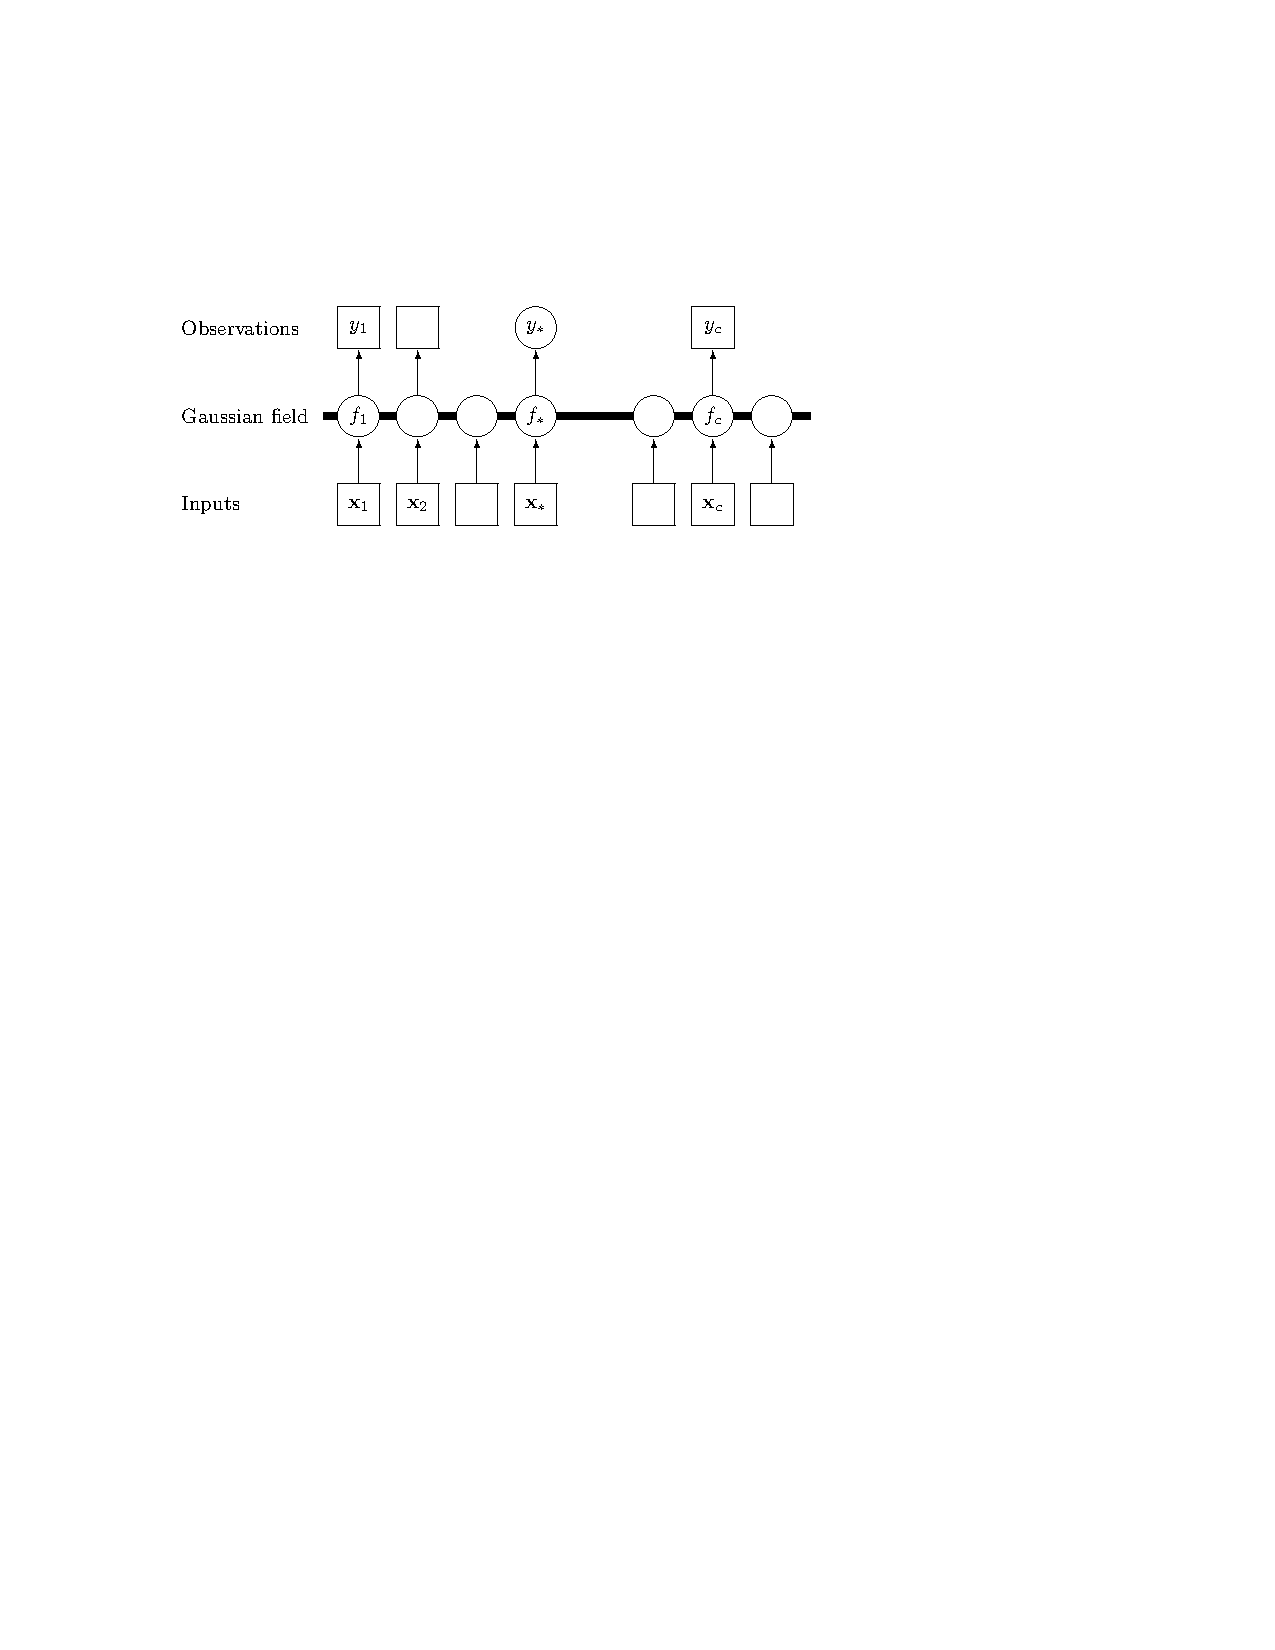
\includegraphics{Regression_model.pdf}
\label{regression_model}
\caption{The relation between input ($x$), observational output ($y$), and the latent variable ($f$). \newline Figure from \cite{RW}}
\end{figure}


\subsection{MLE and MAP for Setting Hyperparameters}
Although Gaussian Process is non-parametric, we still need to find the hyperparameters which define the mean and covariance functions. In fact, the objective of finding hyperparameters other than the parameters for model itself gives us more freedom in defining the distribution function. 

According to Baye's rule,

\[\mbox{posterior} = \frac{\mbox{likelihood}\times \mbox{prior}}{\mbox{marginal likelihood}}\]

if $\theta$ is the collection of all hyperparameters

\[p(\theta|X,y) = \frac{p(y|X,\theta)p(\theta)}{p(y|X)}\]

where the marginal likelihood $p(y|X)$ is given by 

\begin{equation}
\label{pY_X}
p(y|X) = \int{p(y|X,\theta)p(\theta)}d\theta
\end{equation}

The MLE and MAP estimates the integrals by approximating the likelihood $p(y|X,\theta)$ and posterior $p(\theta|X,y)$ respectively as delta function of $\theta$. Indeed, the differences between the approximation and the real function value may have an negative impact on our final results. However, as the approximations are on hyperparameters, which only affects mean and covariance function but not the function parameters (function values), the negative impact arisen from MLE or MAP is reduced as they propagate to the actual function values.

Note that in equation (\ref{pY_X}), $\theta$ is marginalised out therefore $p(y|X)$ is independent of the values of theta. The maximum a posterior estimate of $\theta$ happens when $p(\theta|X,y)$ is maximised. Since $p(\theta|X,y)$ is proportional to $p(y|X,\theta)$, if we have little knowledge about the prior information of $\theta$, finding the maximum of the posterior is equivalent to obtaining the value of $\theta$ that maximises $p(y|X,\theta)$. $p(y|X,\theta)$ can be written as the integration of latent variable f

\begin{equation}
\label{theta_likelihood}
p(y|X,\theta) = \int{p(y|f,X,\theta)p(f|X,\theta)}df
\end{equation}

In Gaussian Process model we assume that $p(f|X,\theta)$ is a Gaussian with mean 0 and variance $K$. A multi-variate Gaussian probability density function can be written as 

\[\mathcal{N}(\mathbf{x},\mathbf{\mu},\mathbf{\Sigma}) = \frac{1}{\sqrt{|2\pi\mathbf{\Sigma}|}}\operatorname{exp}\left(-\frac{1}{2}(\mathbf{x} - \mathbf{\mu})^T\mathbf{\Sigma}^{-1}(\mathbf{x} - \mathbf{\mu})\right)\]

therefore we have

\begin{equation}
\label{f_posterior}
\operatorname{log}p(f|X,\theta) = -\frac{1}{2}f^TK^{-1}f-\frac{1}{2}\operatorname{log}|K| - \frac{n}{2}\operatorname{log}2\pi
\end{equation}

also we know that $y|f\sim \mathcal{N}\left(f,\sigma_n^2 I\right)$, combining it with the above equation we get

\begin{equation}
\operatorname{log}p(y|X,\theta) = -\frac{1}{2}y^T(K+\sigma_n^2 I)^{-1}y - \frac{1}{2}\operatorname{log}\left|K+\sigma_n^2 I\right|- \frac{n}{2}\operatorname{log}2\pi
\end{equation}

This is the final objective function to be maximised. It is also consistent with the covariance of y we derived earlier in equation (\ref{cov_y}) where a noise term is added to the diagonal of $K$.


\subsection{Predictions}
After finding the optimised hyperparameters, predictions can be made by substituting the new inputs into the Gaussian Process model defined by mean and covariance function with the optimised parameters. The joint distribution of training data with no noise can be written as 

\begin{equation}
\left[\begin{array}{c} 
\mathbf{f} \\
\mathbf{f}_\ast \end{array}
 \right] \sim \mathcal{N} 
 \left(\mu(X), \left[\begin{array}{cc}
 K(X, X) & K(X, X_\ast)\\
 K(X_\ast, X) & K(X_\ast, X_\ast)
 \end{array}\right]\right)
\end{equation} 

Where $\mathbf{f}_\ast$ denotes the predictions in $f$ domain. Similarly, distribution of noisy training data can be expressed as

\begin{equation}
\left[\begin{array}{c} 
\mathbf{y}\\
\mathbf{f}_\ast \end{array}
 \right] \sim \mathcal{N} 
 \left(\mu(X), \left[\begin{array}{cc}
 K(X, X) + \sigma_n^2I & K(X, X_\ast)\\
 K(X_\ast, X) & K(X_\ast, X_\ast)
 \end{array}\right]\right)
\end{equation}

Then the distribution of $\mathbf{f}_\ast$ conditioned on $X, X_\ast$ and $\mathbf{f}$ follows a Gaussian with mean and variance as below

\begin{align}
\label{predictive_mean_noise_free}
\bar{\mathbf{f}}_\ast & = \mu(X_\ast) + K(X_\ast, X)K(X,X)^{-1}(\mathbf{f} - \mu(X))
\\
\label{predictive_covariance_noise_free}
\operatorname{cov}(\mathbf{f}_\ast) & = K(X_\ast, X_\ast) - K(X_\ast, X)K(X, X)^{-1}K(X, X_\ast)
\end{align}
 
and the noisy version,
\begin{align}
\bar{\mathbf{f}}_\ast & = \mu(X_\ast) + K(X_\ast, X)[K(X,X) + \sigma_n^2I]^{-1}(\mathbf{y} - \mu (X))
\\
\operatorname{cov}(\mathbf{f}_\ast) & = K(X_\ast, X_\ast) - K(X_\ast, X)[K(X,X) + \sigma_n^2I]^{-1}K(X, X_\ast)
\end{align}

\begin{figure}[h]

\centering
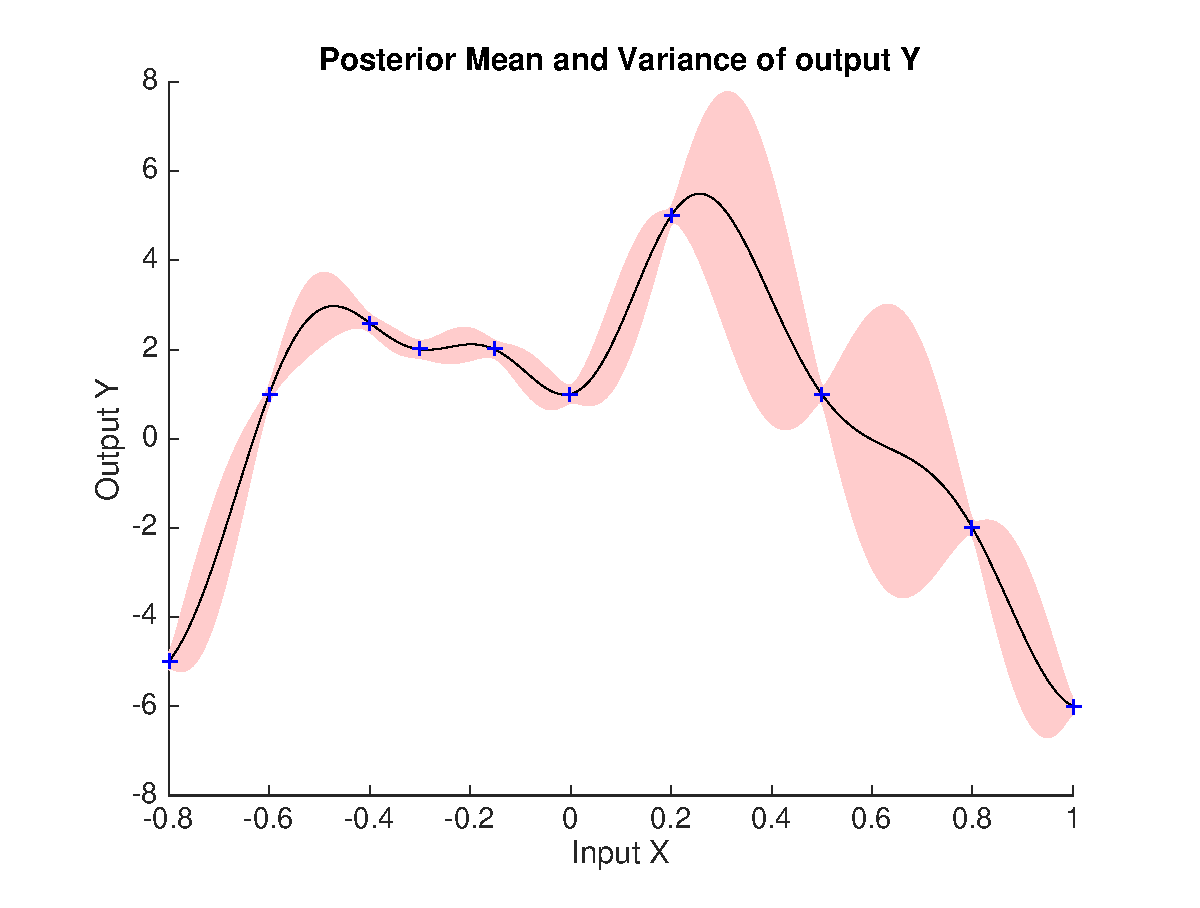
\includegraphics[scale = 0.5]{RegressionPlot1D.eps}
\label{regression_1D_plot}
\caption{Example plot of Regression with 1D input and output. Blue points represent the training set. Red region represents the variance of prediction. Note that the variance at the training points is almost reduced to zero as there is little uncertainty at these points (they are actually zero in noise free cases). The further way from training points, the more uncertain predictions become.}
\end{figure}

\subsection{Computational Issues}

\subsubsection{Conditioning on K}
Because of the requirement for $K$ to be invertible, $K$ has to be full rank. However, when the input data is so closed to each other compared to the length scale used, adjacent rows in $K$ might become the same under limited significant figures, making the matrix not full rank anymore.

This problem is avoided in regression problems by adding noise. While in classification problems that we are going to talk about later, artificial noise, also called jitters, has to be added. The amount of jitters needed differs by data, and user is required to adjust its size until $K$ becomes positive definite.

\subsubsection{Cholesky Decomposition}
For large data sets, Gaussian Process can be very slow. The computation on large covariance matrix makes it highly time consuming. The most expensive computation is the inversion of $K$. Cholesky decomposition is one way to tackle this problem. It decomposes a positive definite matrix into product of two triangular matrices

\begin{equation}
K = LL^T = U^TU
\end{equation}

where $L$ is a lower triangular matrix and $U$ is an upper triangular matrix. The inverse of $K$ can simply be computed by

\begin{equation}
K^{-1} = L^{-T}L^{-1} = U^{-1}U^{-T}
\end{equation}

It is much faster to compute the inverse of a triangular matrix, giving a reduction in computation complexity from $\mathcal{O}(n)$ to $\mathcal{O}(\frac{1}{2}n)$\cite{marelli2015distributed}. In addition, matrix inversion based on cholesky decomposition is more numerically stable.  


\subsubsection{Partial Derivatives of Hyperparameters}
To optimise the hyperparameters using Newton's method, we need to compute the gradients of log likelihood of $\theta$ wrt. the hyperparameters $\theta_i$, given by 
 
\begin{equation}
\begin{split}
\frac{\partial}{\partial \theta_i} \operatorname{log}p(y|X,\theta) & = \frac{1}{2}y^T K^{-1}\frac{\partial K}{\partial \theta_i}K^{-1}y \, - \, \frac{1}{2}tr(K^{-1}\frac{\partial K}{\partial \theta_i}) \\ & = \frac{1}{2}tr\big( (\alpha\alpha^T - K^{-1})\frac{\partial K}{\partial \theta_i}\big) \quad\quad\quad \mbox{where}\quad\alpha = K^{-1}y
\end{split}
\end{equation}

One thing to notice is that many of the parameters, such as lengthscale and frequency, are always positive. Therefore it is more convenient to optimise over their logrithms other than themselves. e.g $\theta = \operatorname{log}\theta$ 









\section{Gaussian Process Classification}
\rhead{Classification}
Gaussian Process classification can be simply derived from GP regression except for the fact that outputs are discrete numbers representing class labels instead of continuous numbers in regression. Typically class labels are 1 and -1 for binary class problems. However, we do get a continuous intermediate function before the final label is decided. This is the latent variable on which regression is applied. Then the result of regression will be 'squashed' into range [0,1] to give the probability of a certain class.


\subsection{The 'Squashing' Function}
The 'squashing' function can be any sigmoid function. Two typical sigmoid functions are logistic function $\lambda (f) = 1/(1 + \operatorname{exp}(-y_if_i))$ and cumulative Gaussian function $\Phi (f) $. Inference is hence divided into two steps. First is to compute  the distribution of the prediction latent variable $f_*$ in terms of previous observations 

\begin{equation}
\label{classification_prediction}
p(\boldsymbol f_*|\boldsymbol X,\boldsymbol y,\boldsymbol x_*) = \int p(\boldsymbol f_*|\boldsymbol X,\boldsymbol x_*,\boldsymbol f)p(\boldsymbol f|\boldsymbol X,\boldsymbol y)\ d\boldsymbol f
\end{equation}

where \(p(\boldsymbol f|\boldsymbol X,\boldsymbol y) = {p(\boldsymbol y|\boldsymbol f)p(\boldsymbol f|\boldsymbol X)}/{p(\boldsymbol y|\boldsymbol X)}\) is the posterior of latent variables $\boldsymbol f$, which is estimated by MAP with respect to hyperpamaters($l$ and $\sigma_f$).

Then the probabilistic prediction is estimated by substitute the latent f into sigmoid function and average over 

\begin{equation}
\label{predictive_probability}
\bar{\pi}_* \triangleq p(y_* = +1|X,y,x_*) = \int \sigma (f_*)p(f_*|X,y,x_*) df_*
\end{equation}


\subsection{The Laplace Approximation}

In the case of regression (equation \ref{theta_likelihood}), we assumed that both the likelihood $p(y|f)$ and the posterior over latent variable $p(f|X,\theta)$ are Gaussian. The integral for finding $p(y|X,\theta)$ and the prediction can be computed analytically. However, in classification, the non-Gaussian likelihood and the posterior of latent function make the integral (equation (\ref{classification_prediction})) not analytically tractable. Laplace's approximation can be used to approximate these two terms by doing a second order Taylor 		expansion around its maximum point. 

The Gaussian approximation of the posterior of $f$ can be obtained by:


\begin{equation}\label{LaplaceApp}
q(f|X,y) = \mathcal{N}(f|\hat{f},A^{-1}) \propto \operatorname{exp}(-\frac{1}{2}(f-\hat{f})^T A(f-\hat{f})) \,\sim\, p(f|X,y)
\end{equation}

where $\hat{f} = \operatorname{argmax_f} p(f|X,y)$ and $A = -\bigtriangledown\bigtriangledown \operatorname{log}p(f|X,y)|_{f=\hat{f}}$ is the hessian of negative log posterior.


The reason we choose Laplace's approximation here is that it is more likely to give a better approximation than MLE or MAP\cite{azevedo1994laplace}. Although it may still be inappropriate for the true shape of the data: the peak can be much sharper or flatter than what the approximation described. 

%\begin{equation}\label{LaplaceApp_prediction}
%q(f_*|X,y, x_*) = \mathcal{N}(f|\hat{f},A^{-1}) \propto \operatorname{exp}(-\frac{1}{2}(f-\hat{f})^T A(f-\hat{f})) \,\sim\, p(f_*|X,y, x_*)
%\end{equation}


\section{Implementation}
%%The project is mainly focused on classification problem, where the input is the measurements of each job and the output is the class label indicating whether the job would be automated or not.

\subsection{Optimising the latent variable}
By Baye's rule
\[
p(\boldsymbol f|\boldsymbol X,\boldsymbol y) = {p(\boldsymbol y|\boldsymbol f)p(\boldsymbol f|\boldsymbol X)}/{p(\boldsymbol y|\boldsymbol X)} 
\]

We need to find the $\hat{f}$ that maximises $p(f|X,y)$. Also, $p(y|X)$ is independent of $f$, only the numerator need to be considered. Take the logrithm of $p(f|X,y)$ we get

\begin{equation}
\begin{split}
\Psi(f) & = \operatorname{log}p(f|X,y) \\
& = \operatorname{log}p(y|f) + \operatorname{log}p(f|X) \\
& = \operatorname{log}p(y|f) + \frac{1}{2}f^TK^{-1}f - \frac{1}{2}\operatorname{log}|K| - \frac{n}{2}\operatorname{log}2\pi
\end{split}
\end{equation}

and its derivatives w.r.t. $f$:

\begin{align}
\nabla\Psi(f) & = \nabla\operatorname{log}p(y|f) - K^{-1}f \\
\nabla\nabla\Psi(f) & = \nabla\nabla\operatorname{log}p(y|f) - K^{-1} = -W - K^{-1}
\end{align}

where $W$ is the second derivative of negative log likelihood of $f$. Since we know that $y_i$ depends on $f_i$ only, $W$ is a diagonal matrix. The best latent f can then be found at $\nabla\Psi = 0$, which gives 

\begin{equation}
\label{optimised_f}
\hat{f} = K(\nabla \operatorname{log}p(y|\hat{f}))
\end{equation}

This is a non-linear function therefore can be solved by Newton's method. Commonly used convergence criteria include the difference between successive values of $\Psi (f)$, the magnitude of gradient vector $\nabla\Psi (f)$ or the changes between values of $f$. In practice, the convergence of objective function is assured by checking that each iteration gives an increase in $\Psi (f)$. If not, a smaller step change in $f$ should be used. 

\begin{figure}
\centering
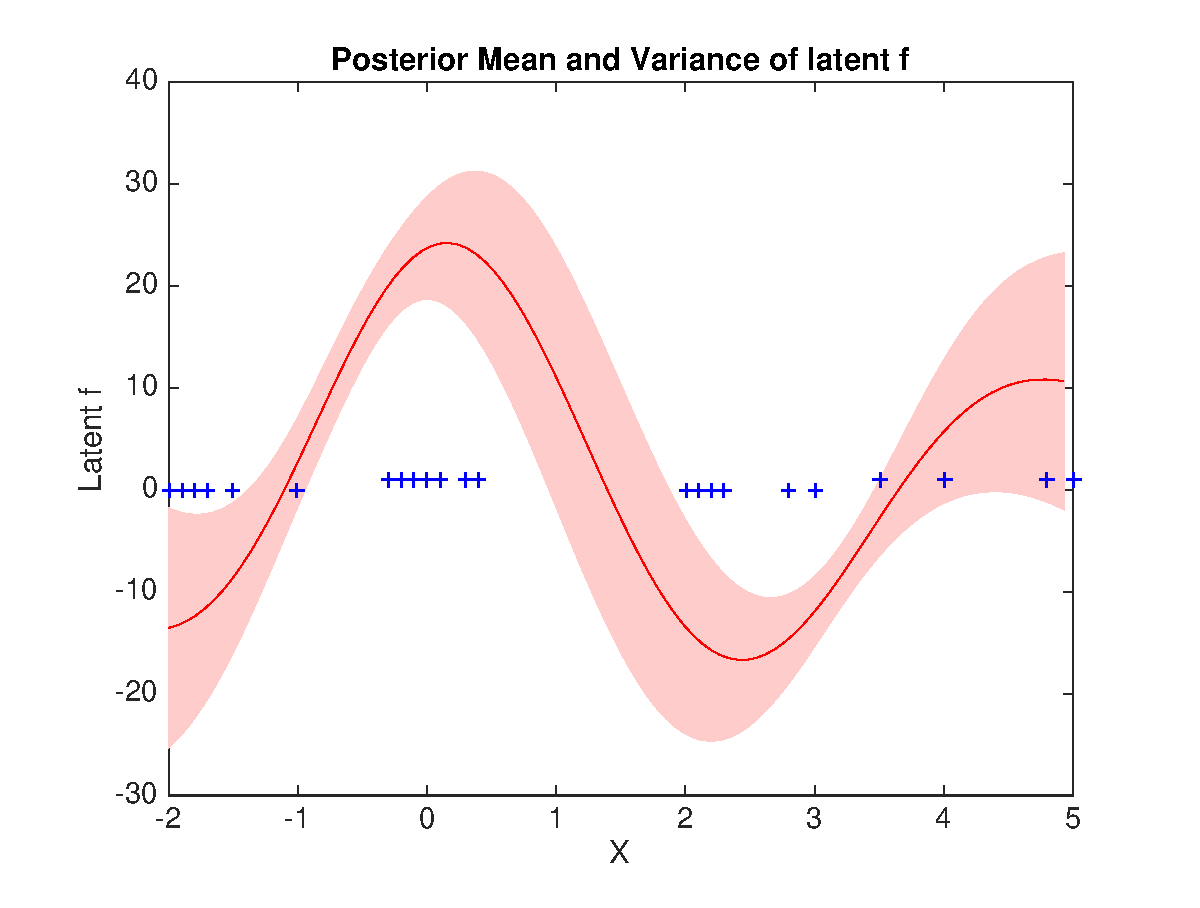
\includegraphics[scale=0.5]{classification_latent_f.eps}
\caption{Example plot of latent variable. Blue crosses are training points and red region is its variance. The variance now is never going to be zero because the latent function value is not told directly. While in noise free regression, the exact value of output at training points is told.}
\end{figure}

\subsection{Maximising the Objective Function}
The objective function here is the log posterior $p(y|X,\theta) = \int p(y|f)p(f|X) df = \int \operatorname{exp}(\Psi(f)) df$ which can be obtained by using Laplace's approximation of $p(f|X,y)$ (Taylor expansion around $\hat{f}$)

\begin{equation}
p(y|X,\theta) \simeq q(y|X,\theta) = exp(\Psi(\hat{f})) \int \operatorname{exp}(-\frac{1}{2}(f - \hat{f})A(f-f\hat{f})) df
\end{equation}
thus
\begin{equation}
\operatorname{log}q(y|X,\theta) = -\frac{1}{2}\hat{f}^TK^{-1}\hat{f} + \operatorname{log}p(y|\hat{f}) - \frac{1}{2}\operatorname{log}|B|
\end{equation}

where $|B| = |I_n + W^{\frac{1}{2}} K W^{\frac{1}{2}}|$ and $K$ is covariance defined by $\theta$. This is the final function we need to run optimisation on. 

\subsubsection{Sampling Methods for Hyperparameters}
In most of the cases, the objective function is non-linear, which means that more than one set of initial hyperparameters has to be assigned as the starting points for optimisation. Following are two methods used for low number of hyperparameters (usually 1 or 2) and higher number of hyperparameters.


Uniform sampling is one of the most common and easily obtainable sampling method. Samples are simply drawn from sample space by dividing the sample space with the number of required samples and taking one in each subspaces (or more strictly, with equal distance between samples). This is usually an idea sampling method for low dimensional problems where the number of dimensions will not largely increase the number of samples if we want to achieve the same number of sampling intervals in each dimension. 

\begin{figure}
\centering
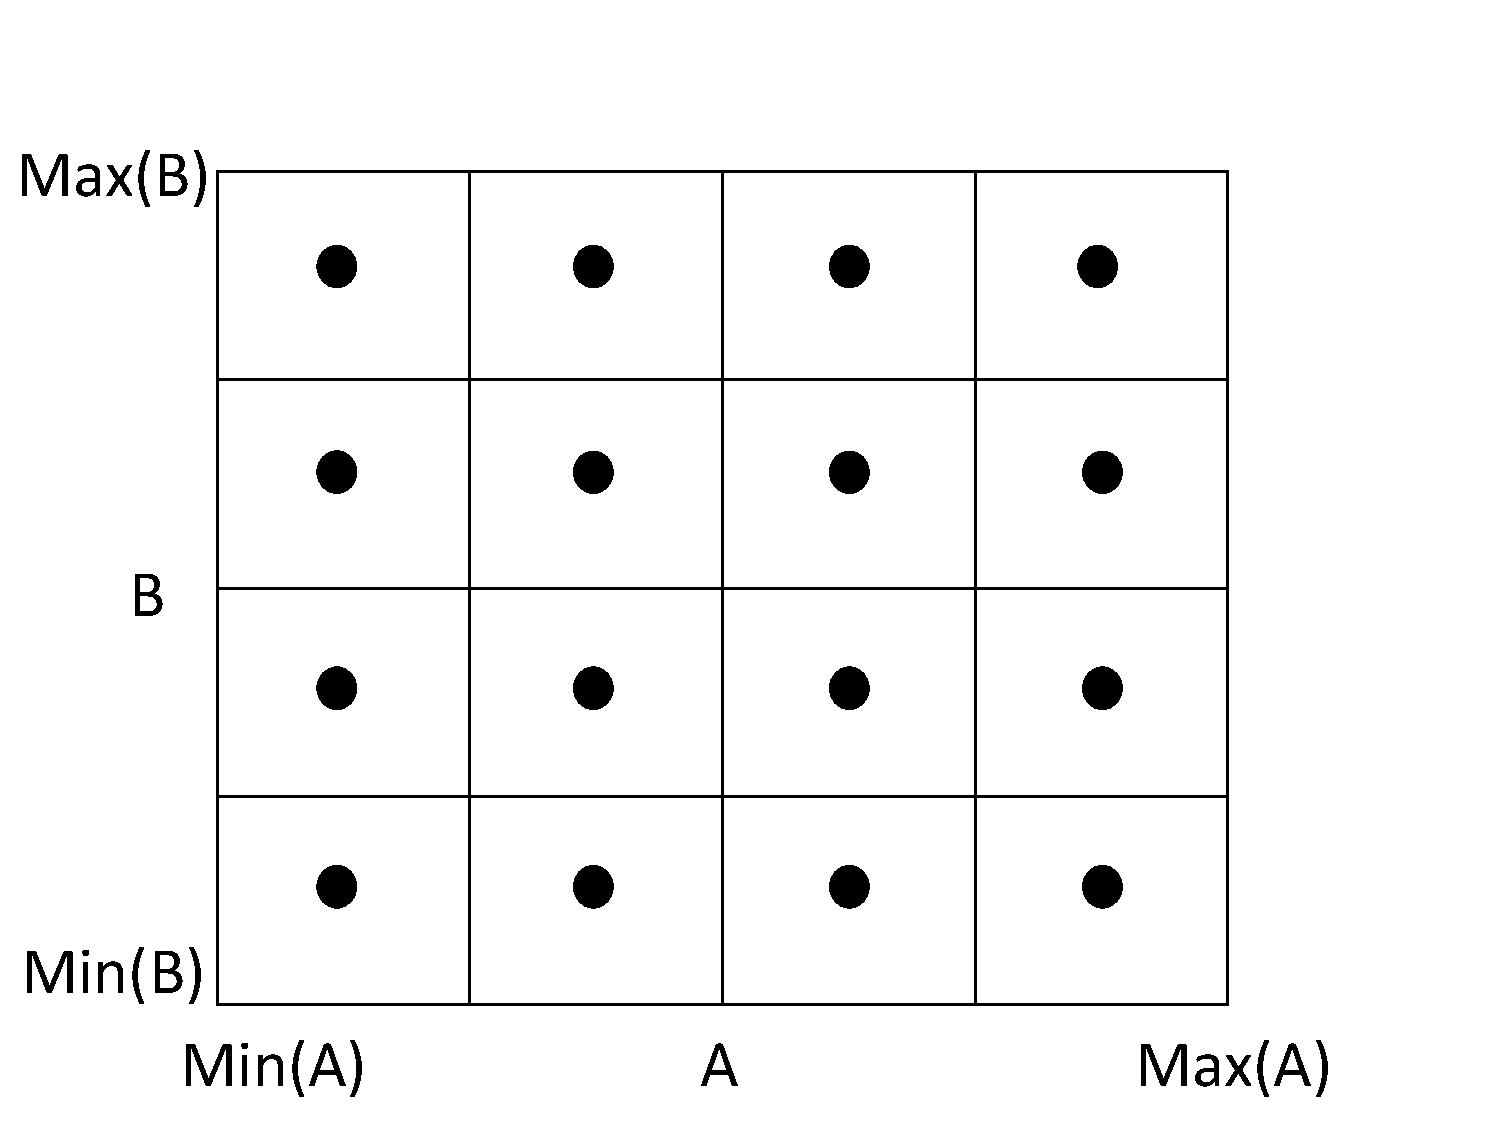
\includegraphics[scale=0.3]{Uniform_sampling.pdf}
\caption{A simple example of 2-dimensional uniform sampling with 4 sampling intervals in each dimension.}
\end{figure}


Latin Hypercube sampling is commonly used for higher dimensional problems. If we want N samples from a one-dimensional variable, we can either uniformly take N points with equal distant from one another, or we can divide the sampling space into N equal intervals and take one sample from each interval. Latin Hypercube Sampling (LHS) is a simple extension from uniform sampling. When taking N samples from a M-dimensional variable, the sampling space of each dimension is divided into N equal intervals. Each interval is sampled once with the order of sampling being random. Then all the samples from M dimensions are combined to give N samples each has M dimensions. Each of the possible combinations of intervals forms a multi-dimensional region that sample could draw from, called a Latin square for two-dimensional sampling space and a Latin hypercube for higher dimensions. 

One advantage of LHS over random sampling is its uniformity. It ensures that samples are well-distributed in each dimension independently. While in random sampling, samples are generated without taking into account the previous samples, they results may be squeezed together, resulting in repeated optimisation results while leaving the other area blank. Non-linear function optimisation means that samples has to be well distributed. The more uniform the samples are, the more likely the global maximum could be found. Another important feature is that LHS does not require more samples for larger dimensions. In uniform sampling, a M-dimensional variable with N samples for each dimension means that N$\times$M samples will be drawn in order to cover the whole sampling space. Obviously for higher dimensional problems this is too time-consuming. For Gaussian process, the hyperparameters involved in optimisation include those used to define mean and covariance functions. When each weighting computing the distance between inputs are treated as hyperparameters, much higher dimensional samples needs to be drawn, leading to a strong preference in Latin Hypercube Sampling.  

\begin{figure}
\begin{subfigure}{0.5\textwidth}
\centering
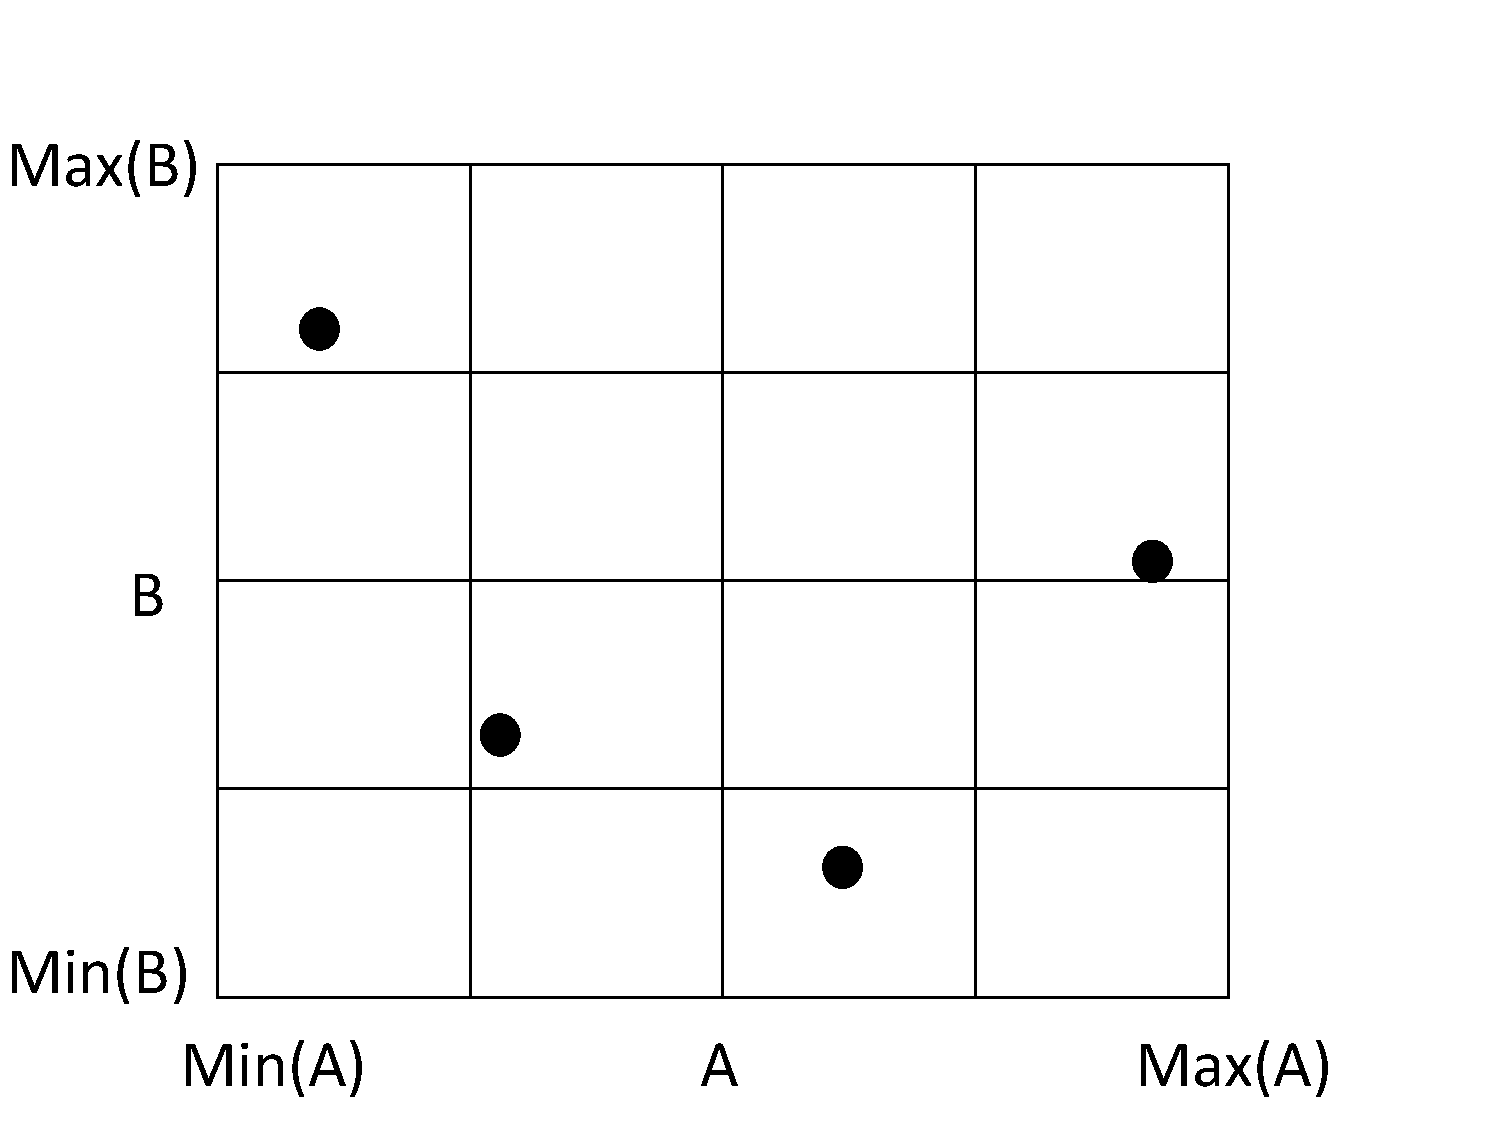
\includegraphics[scale = 0.3]{LHS.pdf}
\caption{Latin Hypercube Sampling}
\end{subfigure}
\hspace*{0.02\textwidth}
\begin{subfigure}{0.5\textwidth}
\centering
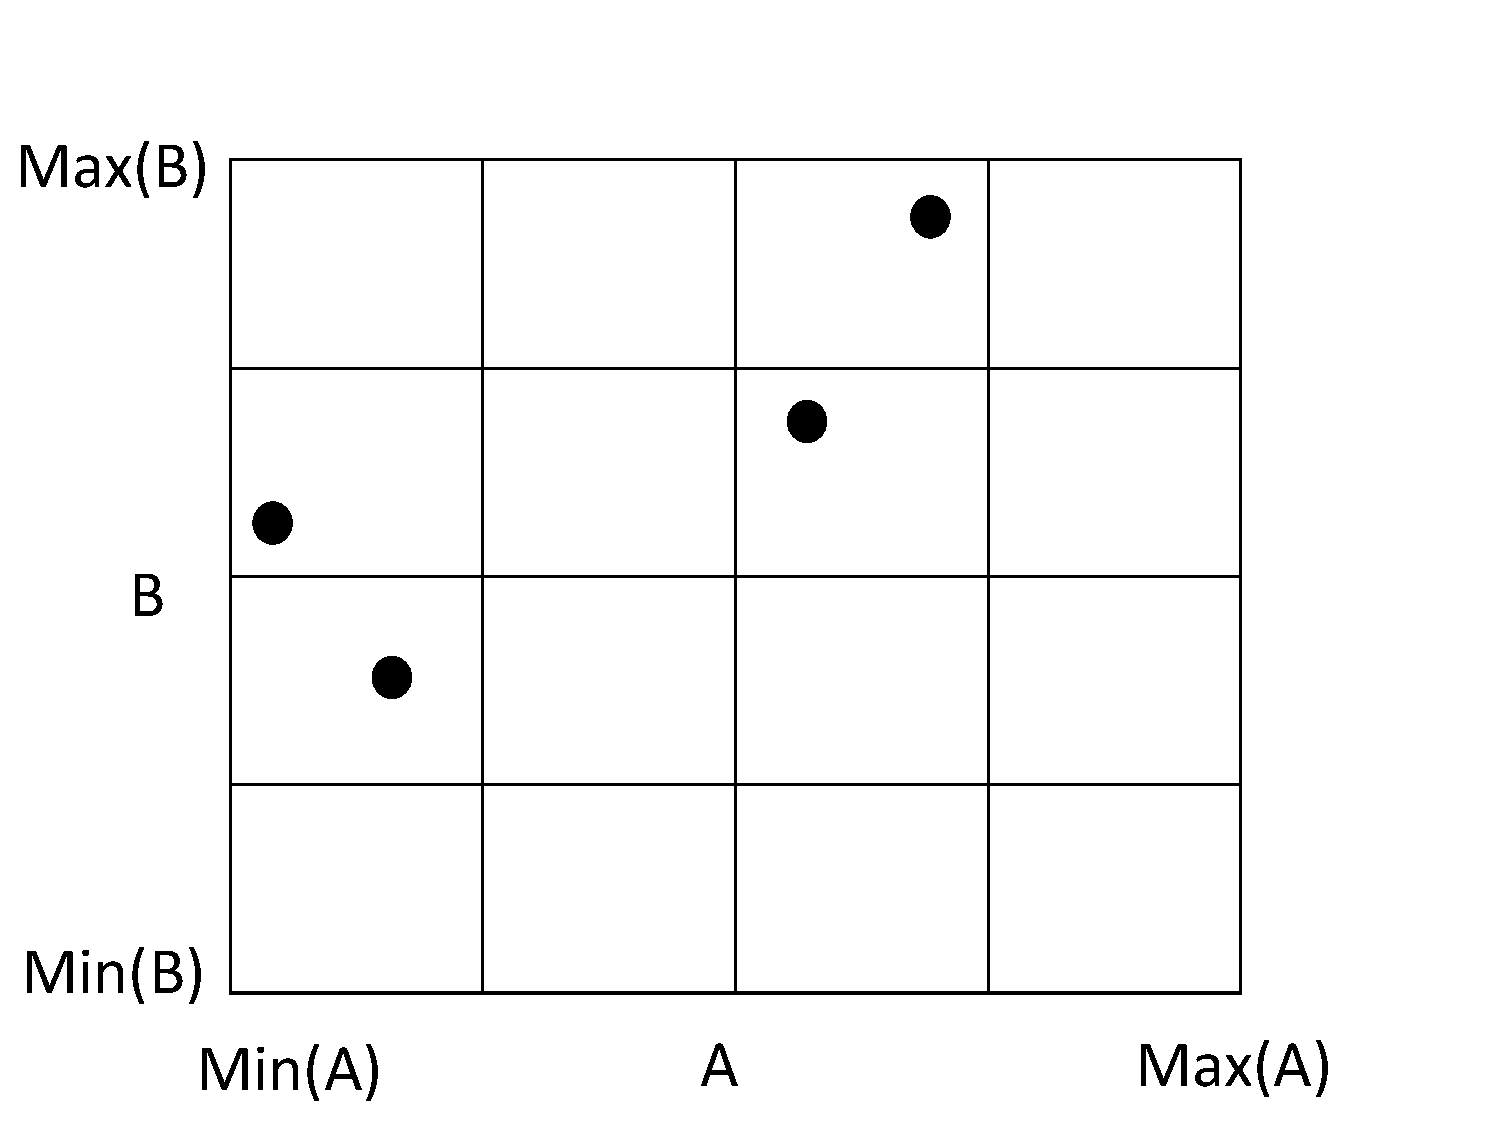
\includegraphics[scale = 0.3]{RS.pdf}
\caption{Random Sampling}
\end{subfigure}
\caption{Comparison between Latin Hypercube sapling and random sampling. Although Latin hypercube sampling may not represent the most variable overall (which can be improved by Orthogonal sampling), it gives a pretty good variability in each dimension. Random sampling does not secure any variability. }
\end{figure}



\subsubsection{Derivatives of Hyperparameters}

Again, as in regression, we need to find the gradient of likelihood w.r.t. all the hyperparameters we are trying to optimise. The case is slightly more difficult than regression as we introduced a latent variable $f$ and used Laplace's Approximation for likelihood itself. 

Since covariance matrix $K$ is a function of hyperparameters, therefore $\hat{f}$ and $W$ are implicit functions of hyperparameters. The derivative of equation (\ref{LaplaceApp}) is


\begin{equation}
\frac{\partial \operatorname{log}q(y|X,\theta)}{\partial \theta_i} = \frac{\partial \operatorname{log}q(y|X,\theta)}{\partial \theta_i}\bigg|_{explicit} + \sum_{i=1}^n \frac{\partial \operatorname{log}q(y|X,\theta)}{\partial \hat{f}_i}\frac{\partial \hat{f}_i}{\partial \theta_i}
\end{equation}

where


\begin{align} 
\label{eq:al1}
\frac{\partial \operatorname{log}q(y|X,\theta)}{\partial \theta_i}\bigg|_{\operatorname{explicit}} &= \frac{1}{2}\hat{f}^T K^{-1}\frac{\partial K}{\partial \theta_i}K^{-1}\hat{f} - \frac{1}{2}tr\Big((W^{-1}+K)^{-1}\frac{\partial K}{\partial \theta_i}\Big) \\ 
\label{eq:al2}
\frac{\partial \operatorname{log}q(y|X,\theta)}{\partial \hat{f}_i} &= -\frac{1}{2} \big[(K^{-1}+W)^{-1}\big]_{ii}\frac{\partial^3}{\partial f_i^3}\operatorname{log}p(y|\hat{f})
\end{align}



\subsection{Predictive Probability}
Predictive mean can be decided under Laplace's approximation by combining the prediction in regression eq. (\ref{predictive_mean_noise_free}) with eq. (\ref{optimised_f})

\begin{equation}
\label{predictive_mean_classification}
\mathbb{E}[f_\ast|X,y,x_\ast] = K(X_\ast, X)K(X, X)^{-1}\hat{f} = K(X_\ast, X) \nabla\operatorname{log}p(y|\hat{f}) 
\end{equation}

Predictive variance consists of two terms: one from $f_\ast$ given $f$, the other from our estimation of $f$

\begin{equation}
\label{predictive_var_classification}
\mathbb{V}[f_\ast|X,y,x_\ast] = \mathbb{E}[(f_\ast - \mathbb{E}[f_\ast|X,y,x_\ast])^2] + \mathbb{E}[(\mathbb{E}[f_\ast|X,x_\ast,f] - \mathbb{E}[f_\ast|X,y,x_\ast])^2]
\end{equation}

using the matrix inversion lemma\cite{woodbury1950inverting} we get

\begin{equation}
\mathbb{V}[f_\ast|X,y,x_\ast] = K(x_\ast,x_\ast) - K(x_\ast,X)(K(X,X) + W^{-1})^{-1}K(X,x_\ast)
\end{equation}

Predictive probability the new output belong to class 1 is then computed by eq. (\ref{predictive_probability}) except that the distribution of $f_\ast$ is now the result of Laplace's approximation with mean and variance as stated above. 

\begin{equation}
\bar{\pi}_* \triangleq p(y_* = +1|X,y,x_*) = \int \sigma (f_*)q(f_*|X,y,x_*) df_*
\end{equation}

One may argue that expectation of the prediction could be simply equal to the sigmoidal mean of $f_*$. These are actually two different things because of the non-linearity of sigmoid function, the first is averaged probability $E[\pi_*|X,y,x_*]$ while the later one is MAP prediction $\sigma (E[f_*|y])$. Although the final class labels assigned are the same for both cases, only the averaged probability gives the statistically correct results. 

\begin{figure}

\begin{subfigure}{0.48\textwidth}
\centering
	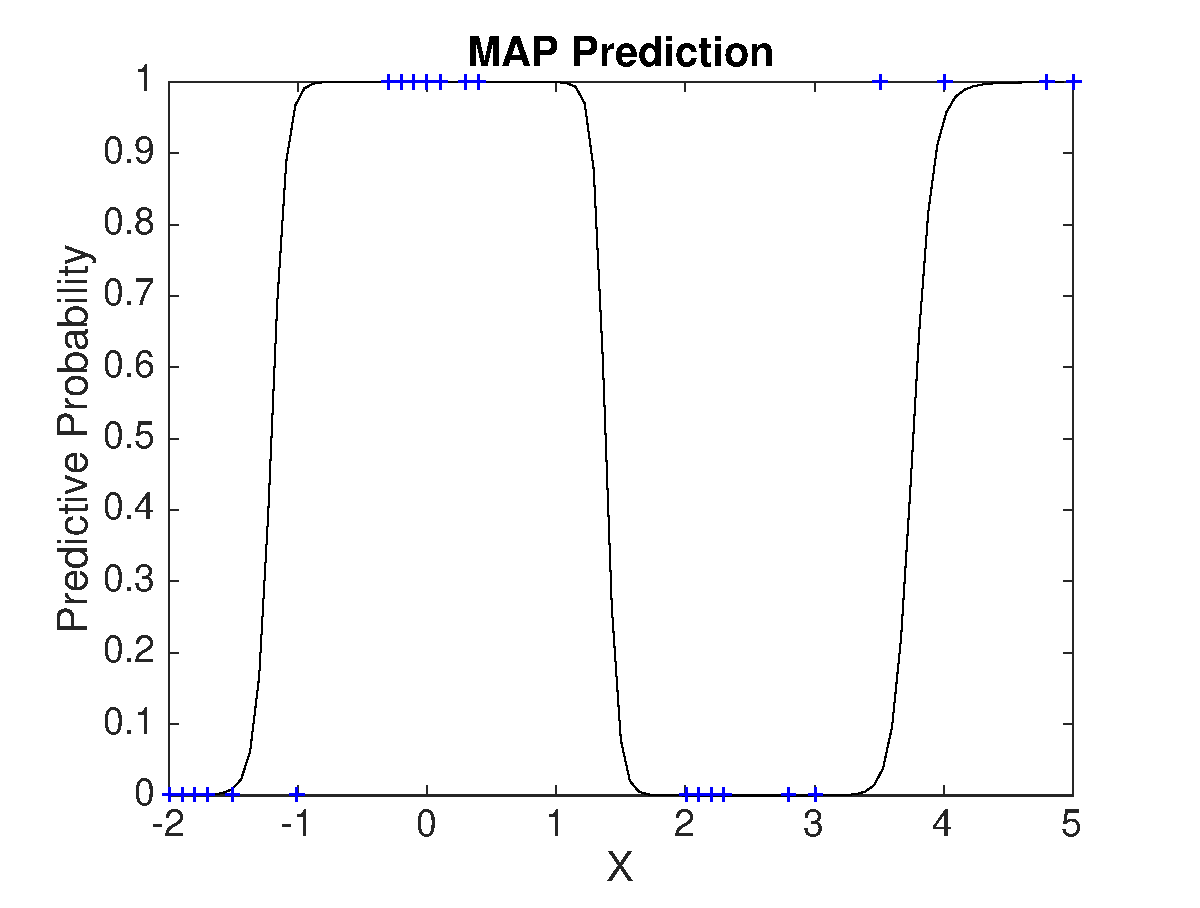
\includegraphics[scale = 0.4]{classification_MAP.eps}
	\caption{}
\end{subfigure}
\hspace*{0.05\textwidth}
\begin{subfigure}{0.48\textwidth}
\centering
	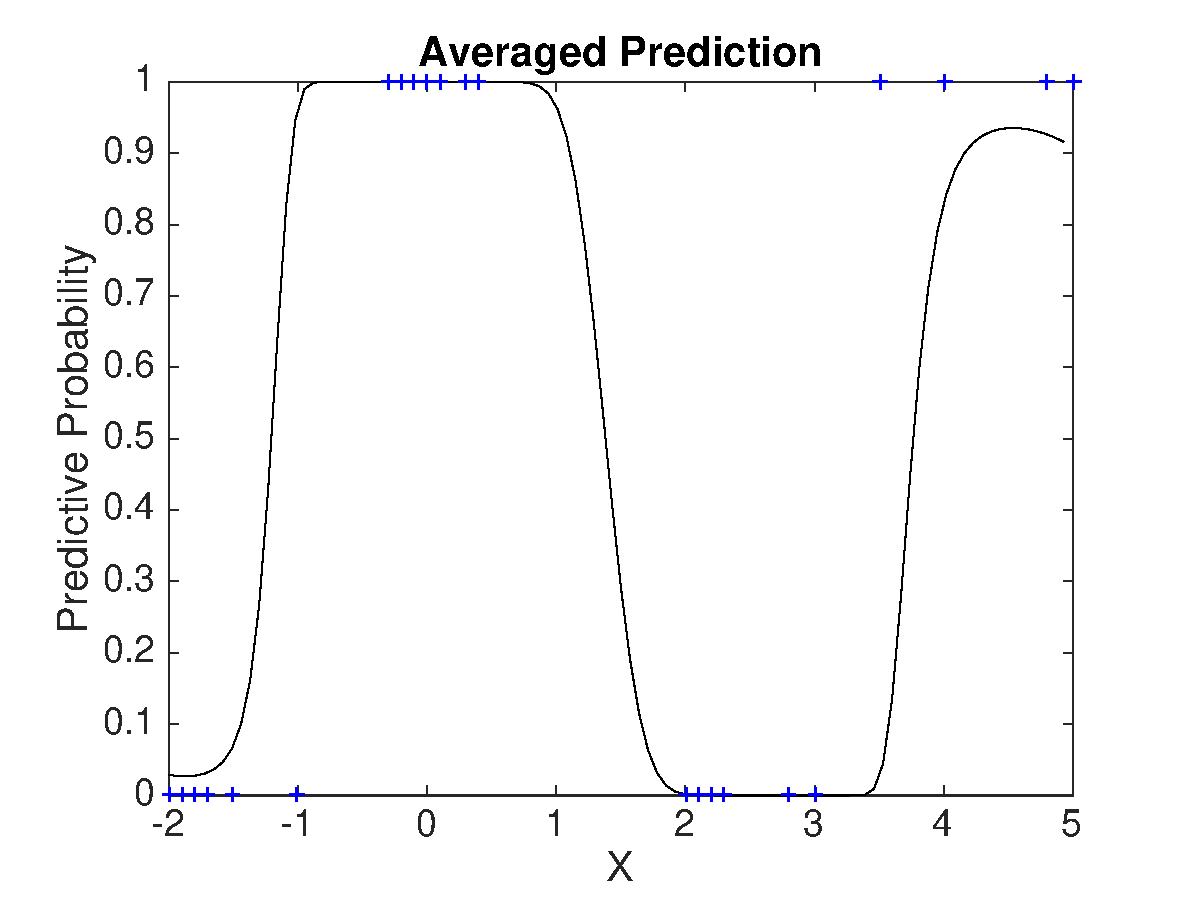
\includegraphics[scale = 0.4]{classification_ave.eps}
	\caption{}
\end{subfigure}

\caption{(a) the MAP prediction. (b) the averaged probability prediction. Blue crosses are training points (class label 1 and -1 but marked as 1 and 0 for better display). The MAP prediction goes to the extremes quicker while the averaged probability is more moderate and tend to be affected by adjacent points}


\end{figure}

\chapter{Gaussian Process for Employment Prediction}
To integrate Gaussian process into the prediction of occupational automatability, we first define the occupational descriptors as the input and the probability of being automated in the future as the output. Hand-labelled training data\cite{frey2013future} which has 33 occupations with label '0'(not possible to be automated) and 37 of them with label '1'(highly possible to be automated). 

Squared exponential is chosen as the covariance function as the output is not expected to have any periodicity but a general smoothness would be helpful (occupations with similar descriptors should have a similar probability of being automated). 







The classifier is first tested by splitting the training set into two groups each with 35 instances, and using one group for training, the other for comparison. The result of the classification on the second group is compared with its true labels by plotting a ROC curve. 

ROC (short for Receiver Operating Characteristic) is a popular tool for performance measurements in binary classification. It is the plotting of true positive rate against false positive rate. One particular interpretation of the curve is its Area Under Curve (AUC). In normalised form, AUC is equal to the probability that a classifier will justify a class 1 object more likely to be class 1 than an object from the other class. The higher the value of AUC, the better the classifier.

\begin{figure}
\centering
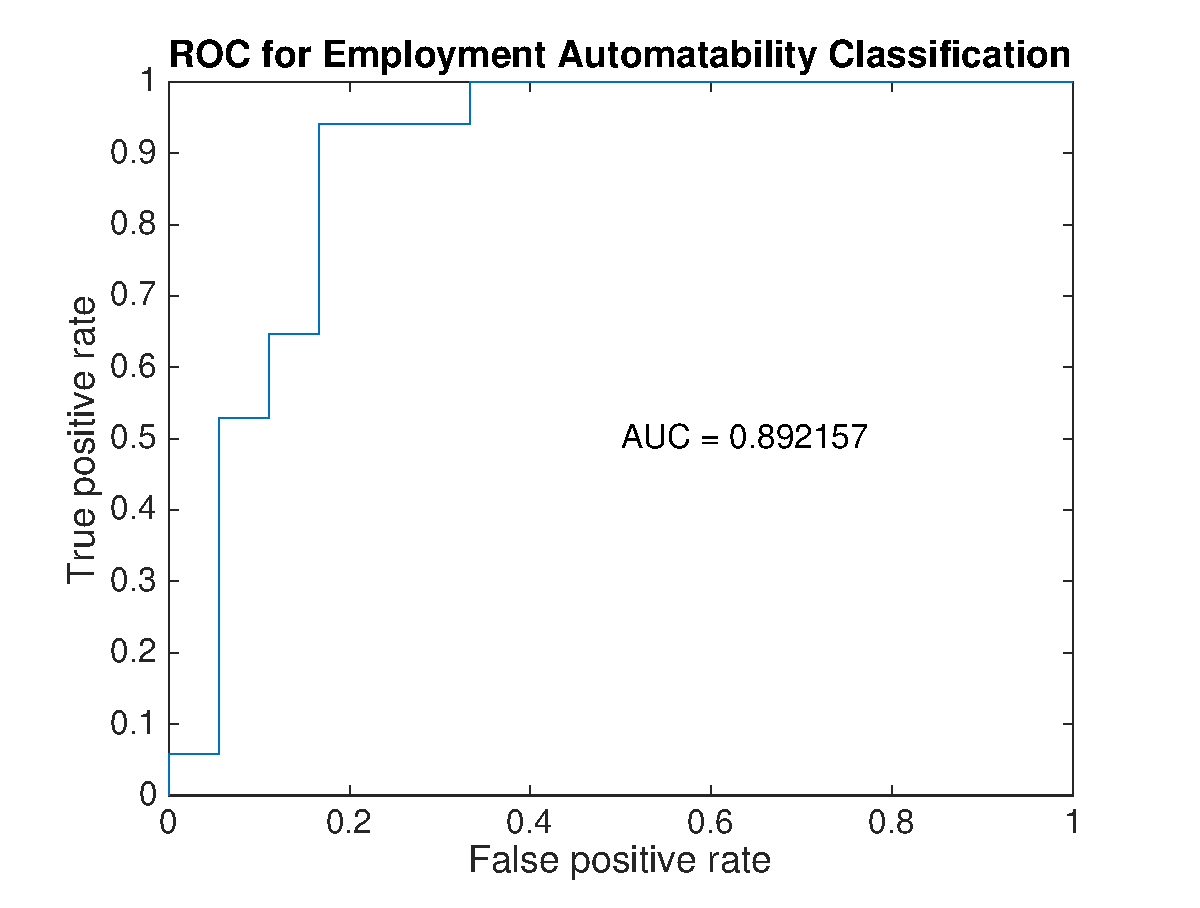
\includegraphics[scale=0.5]{ROC1.eps}
\caption{A typical ROC curve plotted with 35 training data. }
\end{figure}



\newpage

\bibliographystyle{unsrt}
\bibliography{4YP}


\end{spacing}
\end{document}